%% Included in decks: slidemage-manual
%%

% SlideMage manual, chapter "Frame types": figureframe, the frame for a slide
% that is just a figure. The code panel is a zero-space overlay on the Right
% Margin (\cornerfigure with arbitrary content), so the figure itself is
% placed exactly as on a real figure slide.
\setSlideVersion{1-0-0}
\begin{figureframe}{Figure only: \SMCode{figureframe}}
	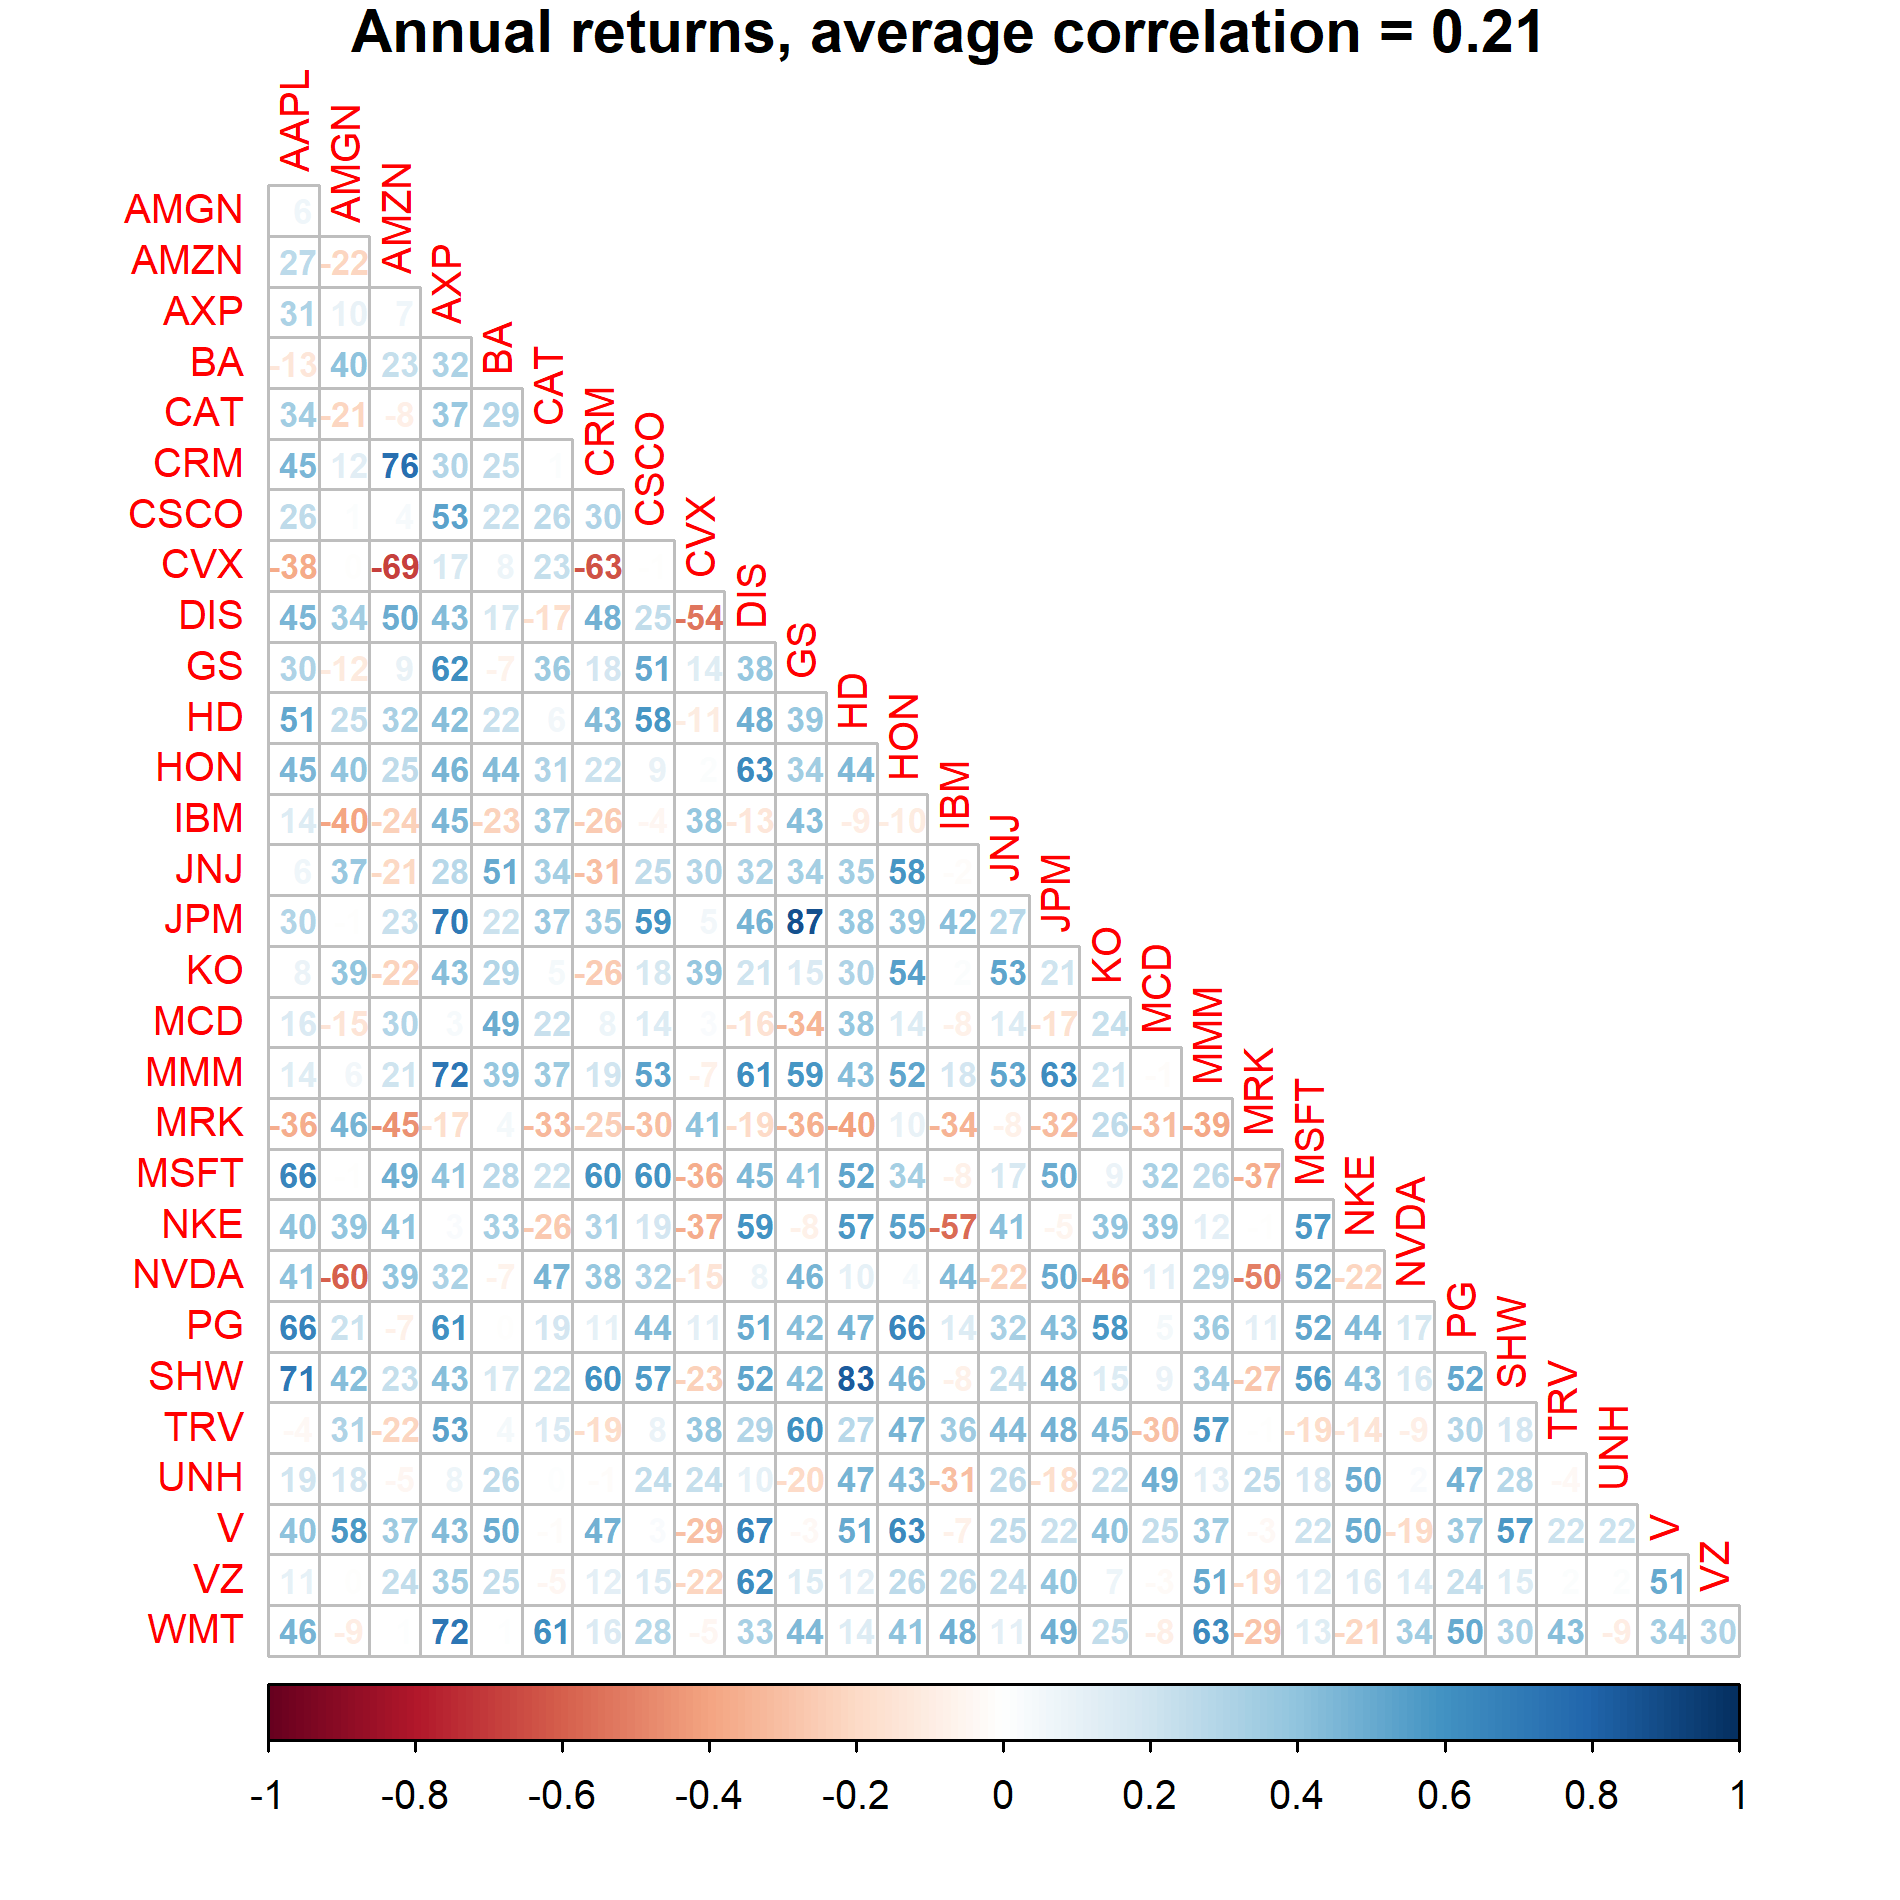
\includegraphics[height=0.64\textheight]{media/correlation-matrix-example.png}
	\cornerfigure[corner=ne]{\begin{minipage}{0.4\linewidth}\small\raggedright\SMLineTop
		A \SMCode{figureframe} holds one figure and nothing else, placed below
		the title bar on the left, or centered: for a chart or picture that needs
		the whole slide.\par\medskip
		\SMCodeFile{snippets/1rb-1.tex}\end{minipage}}
\end{figureframe}
